\section{Introduction}

The Helmholtz equation has the general form
\begin{equation}
    \label{eq:general}
    -\nabla^2{u(\underline{x})} - k^2 u(\underline{x}) = f(\underline{x}), \qquad \underline{x} \in \Omega
\end{equation}
and represents a time-independent form of the wave equation after applying the technique of separation of variables. This equation often arises in various physical problems including the study of electromagnetic radiation, seismology, and acoustics.
% TODO: elaborate on the importance of the equation
% TODO: literature review on the numerical schemes

In this study, we will consider the 1-dimensional Helmholtz equation with impedance boundary conditions in the domain $\Omega=[a, b]$
\begin{equation}
    \label{eq:main}
    \begin{aligned}
        -u''(x) - k^2 u(x) = f(x)\\
        -u'(a) - \imath k^2 u(a) = g_a \in \mathbb{C}\\
        +u'(b) - \imath k^2 u(b) = g_b \in \mathbb{C}
    \end{aligned}
\end{equation}
where $k$ is often called the frequency of the equation, as larger values of this parameter result in more oscillating solutions. We will mainly consider \autoref{eq:main} in the domain $[-1,\:+1]$.
% TODO: Why impedance boundary conditions?

With the recent improvements in knowledge and practical aspects of machine learning techniques, and more specifically, deep learning and neural networks, these methods are being successfully implemented in domains and applications such as computer vision, recommender systems, generative models, etc., where they can benefit from the abundance of data and learn the features that best represent the problem. However, in the context of analyzing complex physical, biological, or engineering systems, these methods are facing the challenge of high cost of data acquisition, which forces us to find a way to make decisions in an semi-supervised fashion while retaining the robustness and convergence of the methods. Recent studies in the literature have introduced deep learning frameworks for solving nonlinear partial differential
euqations (PDEs) that have achieved this goal.

Raissi \textit{et. al.} \cite{RAISSI2019686} have introduced the physics-informed neural networks (PINNs) scheme, which uses the prior knowledge that usually stems from the physics of the system in a structured way as a regularization method to narrow the range of the admissible solutions. They consider the general form of a nonlinear PDE as
\begin{equation}
    u_t + N[u; \lambda] = 0, x \in \Omega, t \in [0, T]
\end{equation}
where $u(t, x)$ denotes the unknown solution, $N[.; \lambda]$ is a nonlinear operator parameterized by $\lambda$, and $\Omega$ is a subset which defines the domain of the system. With $f(t, x)$ as the left-hand-side of this equation, the method consists of defining two neural networks for $u(t, x)$ and $f(t, x)$ with shared parameters, and optimizing these parameters based on a suitable loss function that takes into account the initial condition, boundary conditions, and satisfaction of the equation in quadrature points of the domain. They have shown that their method performs well even with small data for several nonlinear PDEs by comparing their results with the exact solution of those equations.

Kharazmi \textit{et. al.} \cite{kharazmi2019variational} have taken the next step by developing a Petrov-Galerkin version of the PINNs by selecting the trial space to be the space of the neural networks and the test space to be the space of trigonometric functions or Legendre polynomials. They introduce the variational physics-informed neural networks (VPINNs) by incorporating the variational residual of the PDE in the loss function of the network. They show that by integrating by parts the integrand part of the variational form, they can reduce the training time of the VPINNs and increase their accuracy compared to PINNs. They obtain the explicit form of the variational residual for shallow neural networks with one hidden layer, and suggest that numerical integration techniques should be employed for deep neural
networks.

The goal of this study is to implement the VPINNs scheme introduced in \cite{kharazmi2019variational} for solving \autoref{eq:main} and to explore the behavior of these networks with different structures, activation functions, etc. and for different parameters of the equation. For this purpose, we will present the variational formulation of \autoref{eq:main} in \autoref{sec:frameworks}. Then, we will proceed with presenting the frameworks of a finite elements scheme and a VPINN scheme in \autoref{sec:femframework} and \autoref{sec:vpinnsframework}, respectively. In \autoref{sec:results}, we will present and discuss the results of the implemented frameworks with various parameters and conditions Section \ref{sec:conclusion} summerizes our conclusions and provides some suggestions for future works.

\section{Frameworks And Methods}\label{sec:frameworks}
** empty **

\subsection{Variational formulation of the Helmholtz problem}\label{sec:variational}

We take the 1-D version of the Helmholtz equation as expressed in \autoref{eq:main}, and test this equation by a arbitrary smooth test function $v \in {H_{0}^{1} }_{(\Omega)}$ with compact support in the domain, to get
\begin{equation}
    \label{eq:tested}
    \int_{\Omega}{{(-u'' - k^2u)}v} = \int_{\Omega}{fv} \qquad \forall v \in {H_{0}^{1} }_{(\Omega)}.
\end{equation}

Integration by parts gives $\int_{a}^{b}{u''v} = [u'v]_{a}^{b} - \int_{a}^{b}{u'v'}$ which could be replaced into \autoref{eq:tested} to eliminate the second derivative from the equation. Doing this, and by setting $u'(a)v(a) = (-g_a-\imath ku(a))v(a)$ and $u'(b)v(b) = (g_b+\imath ku(b))v(b)$, we get the variational formulation of the Helmholtz impedance problem, which is to find $u \in {H^{1} }_{(\Omega)}$ such that $a(u,\:v) = b(v)$ for all $v \in {H_{0}^{1} }_{(\Omega)}$, where $a(u,\:v)$ and $b(v)$ are defind as

\begin{equation}
    \label{eq:varlhs}
    a(u,\:v) = \int_{a}^{b}{u'v'} - k^2 \int_{a}^{b}{uv} - \imath k (u(a)v(a) + u(b)v(b))
\end{equation}
\begin{equation}
    \label{eq:varrhs}
    b(v) = \int_{a}^{b}{fv} + g_a v(a) + g_b v(b)
\end{equation}

\subsection{Framework of the finite elements scheme}\label{sec:femframework}
We descritize the domain $\Omega=[a,\:b]$ by defining $N+1$ basis functions as
\begin{equation}
    \label{eq:fembasisfuncs}
    \varphi_j(x) = \left\{\begin{matrix}
        1 - \frac{N}{2}|x - x_j|, \quad x_{j-1} < x < x_{j+1}
        \\
        0, \qquad \qquad otherwise.
        \end{matrix}\right.
\end{equation}
for $j = 0, \cdots, N+1$. The resulting basis functions with $N=9$ are illustrated in \autoref{fig:fembases}. Let $V_N = span(\varphi_j)_{j=0, \cdots, N+1} \subset H^{1}$ be a finite-dimensional subset of $H^{1}$. We search for solutions in this subspace, and modify the variational version of the Helmholtz impedance problem as finding $u_N \in V_N$ such that $a(u_N,\:v_N) = b(v_N)$ for all $v_N \in V_N$, where $a(u,\:v)$ and $b(v)$ are defind in Equations \ref{eq:varlhs} and \ref{eq:varrhs}, respectively. We can easily see that it is actually sufficient to ensure that the aforementioned equation is satisfied for all the basis functions $\varphi_i,\:i=0, \cdots, N+1$:
\begin{equation}
    \label{eq:femvar}
    a(u_N,\:\varphi_i) = b(\varphi_i)
\end{equation}
Let $u_N \in V_N$ be a linear combination of the basis of $V_N$, $u_N(x) = \sum_{j=0}^{N}{c_j\varphi_j}$. By plugging $u_N$ into \autoref{eq:femvar}, we can verify that the stated problem could be expressed as a linear system of equations $A\underline{c}=\underline{f}$, where
\begin{equation}
    \label{eq:femcoeffs}
    A = \begin{bmatrix}
        a(\varphi_0,\:\varphi_0) & a(\varphi_1,\:\varphi_0) & \cdots & a(\varphi_N,\:\varphi_0) \\
        a(\varphi_0,\:\varphi_1) & a(\varphi_1,\:\varphi_1) & \cdots & a(\varphi_N,\:\varphi_1) \\
        \vdots & \vdots & \ddots & \vdots \\
        a(\varphi_N,\:\varphi_N) & a(\varphi_0,\:\varphi_N) & \cdots & a(\varphi_N,\:\varphi_N)
        \end{bmatrix},
        \quad
        \underline{c} = \begin{bmatrix}
        c_0\\
        c_1\\
        \vdots\\
        c_N
        \end{bmatrix},
        \quad
        \underline{f} = \begin{bmatrix}
        b(\varphi_0)\\
        b(\varphi_1)\\
        \vdots\\
        b(\varphi_N)
        \end{bmatrix}.
\end{equation}
The solution of this system of equations could be calculated using methods such as Gauss-elimination. We don't need any quadrature rule to calculate the integrals in $a(\varphi_j,\:\varphi_i)$ as these result in determined values depending on $i$ and $j$.

\begin{figure}[h]
    \centering
    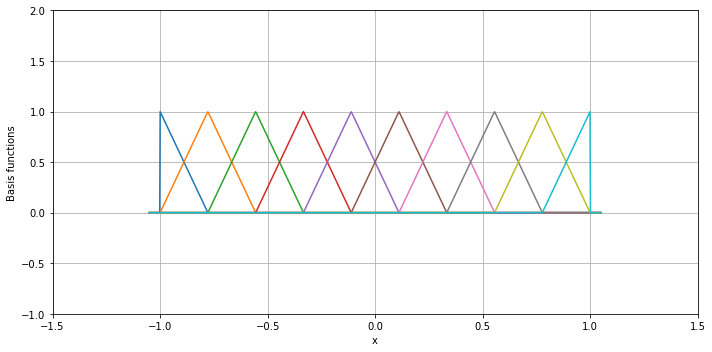
\includegraphics[width = 0.6\textwidth]{img/FEMBasisFunctions.png}
    \caption{The finite element basis functions over the domain $\Omega = [a,\:b]$ for $N=9$.}
    \label{fig:fembases}
\end{figure}

\subsection{Framework and structure of the VPINNs scheme}\label{sec:vpinnsframework}

\subsubsection{Multilayer perceptron}\label{sec:vpinnsmlp}
Let $\mathcal{N}$ be the space of a fully-connected multilayer perceptron (MLP) with 1 node at the input layers, $N$ nodes on each of $D$ hidden layers, and 2 nodes at the output layer as depicted in \autoref{fig:vpinndeepmlp}. The 2 dimensional output represents the real and the imaginary part of the solution $u_N(x) = u_{N,\;1}(x) + \imath u_{N,\;2}(x)$. In case of shallow networks, it could be easily shown that this will be the same as using complex model parameters.\\
For this generic structure of the MLP, each element of the the 2-dimensional solution could be expressed as
\begin{equation}
    \label{eq:vpinngeneric}
    u_{N,\;i} = c_0^i + \sum_{j=1}^{N}{c_j^i \sigma(h^{D} \circ h^{D-1} \circ \cdots \circ h^1(x))},
\end{equation}
where $\sigma (x)$ is a non-linear activation function, $h^1_i = \sigma(w^1_i x + b^1_i)$, and
$h^d_i = \sigma(\sum_{n=1}^{N}{w^d_{i, n} h^{d-1}_n} + b^d_i)$ for $d = 2, \cdots, D$.
\begin{figure}[h!]
    \centering
    \begin{subfigure}[b]{0.45\textwidth}
        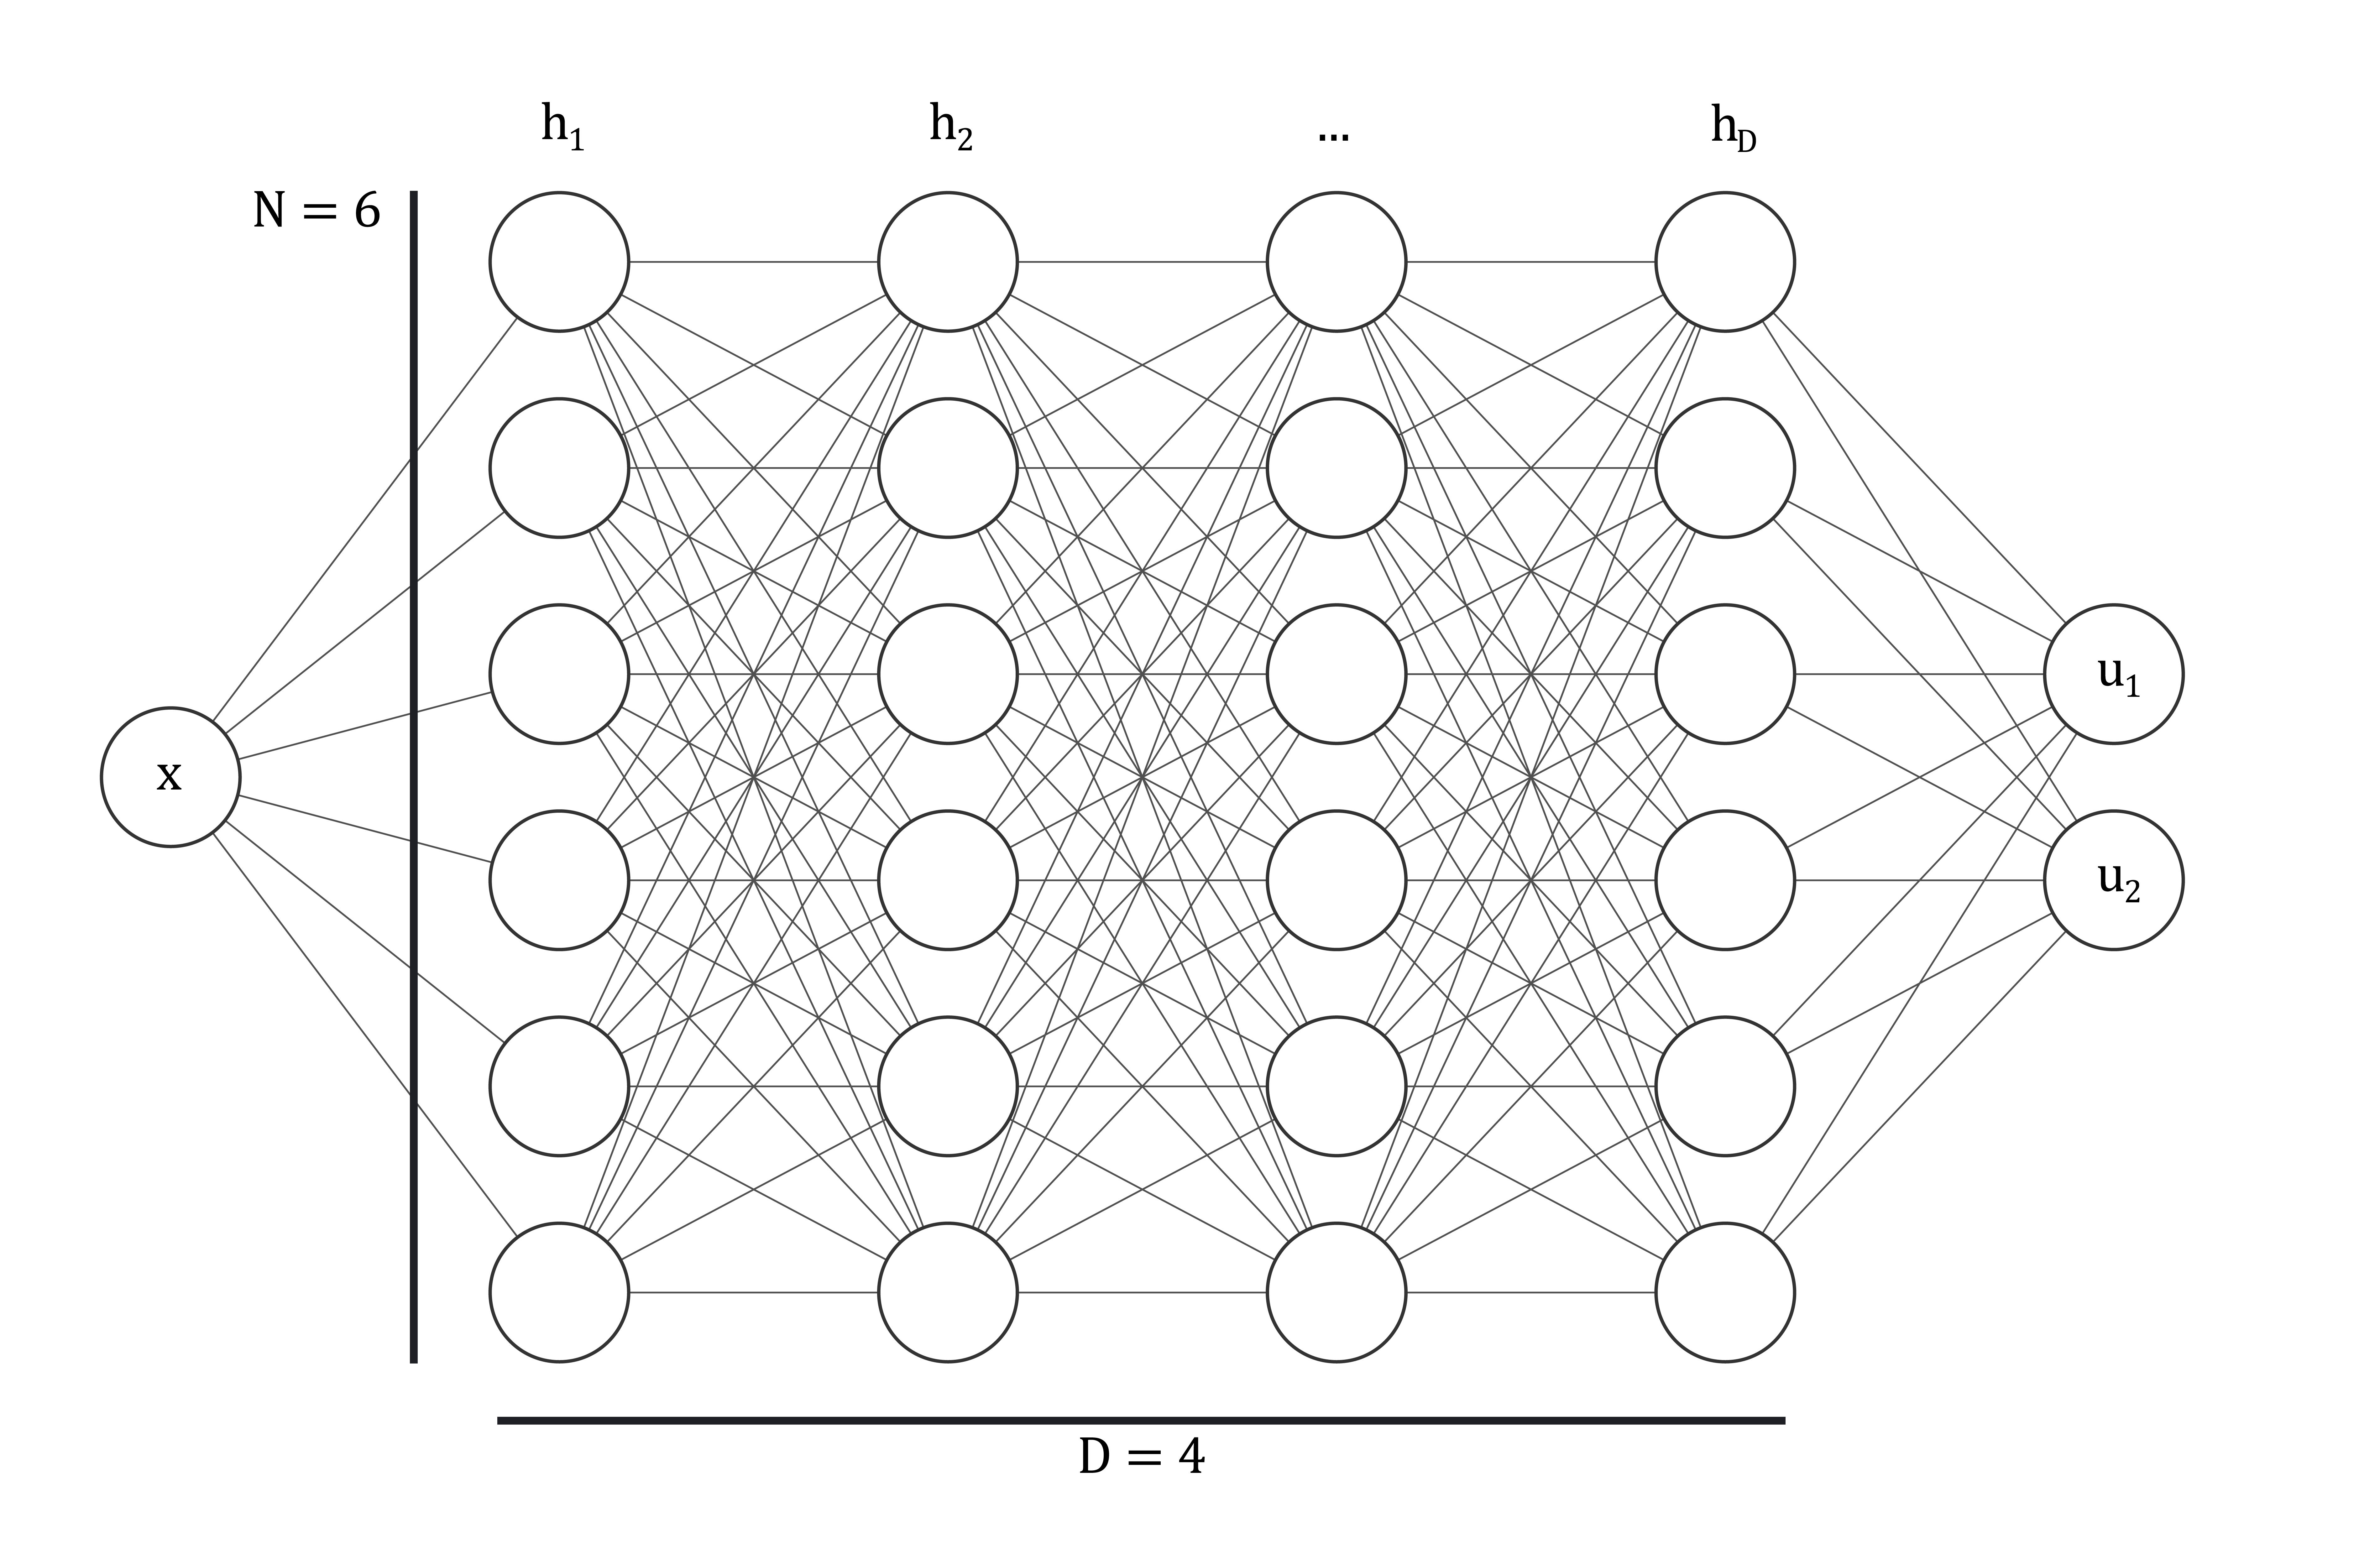
\includegraphics[width=\textwidth]{img/DeepMLP.png}
        \caption{Generic mulilayer perceptron with 4 hidden layer and $N=6$.}
        \label{fig:vpinndeepmlp}
    \end{subfigure}
    \hfill
    \begin{subfigure}[b]{0.45\textwidth}
        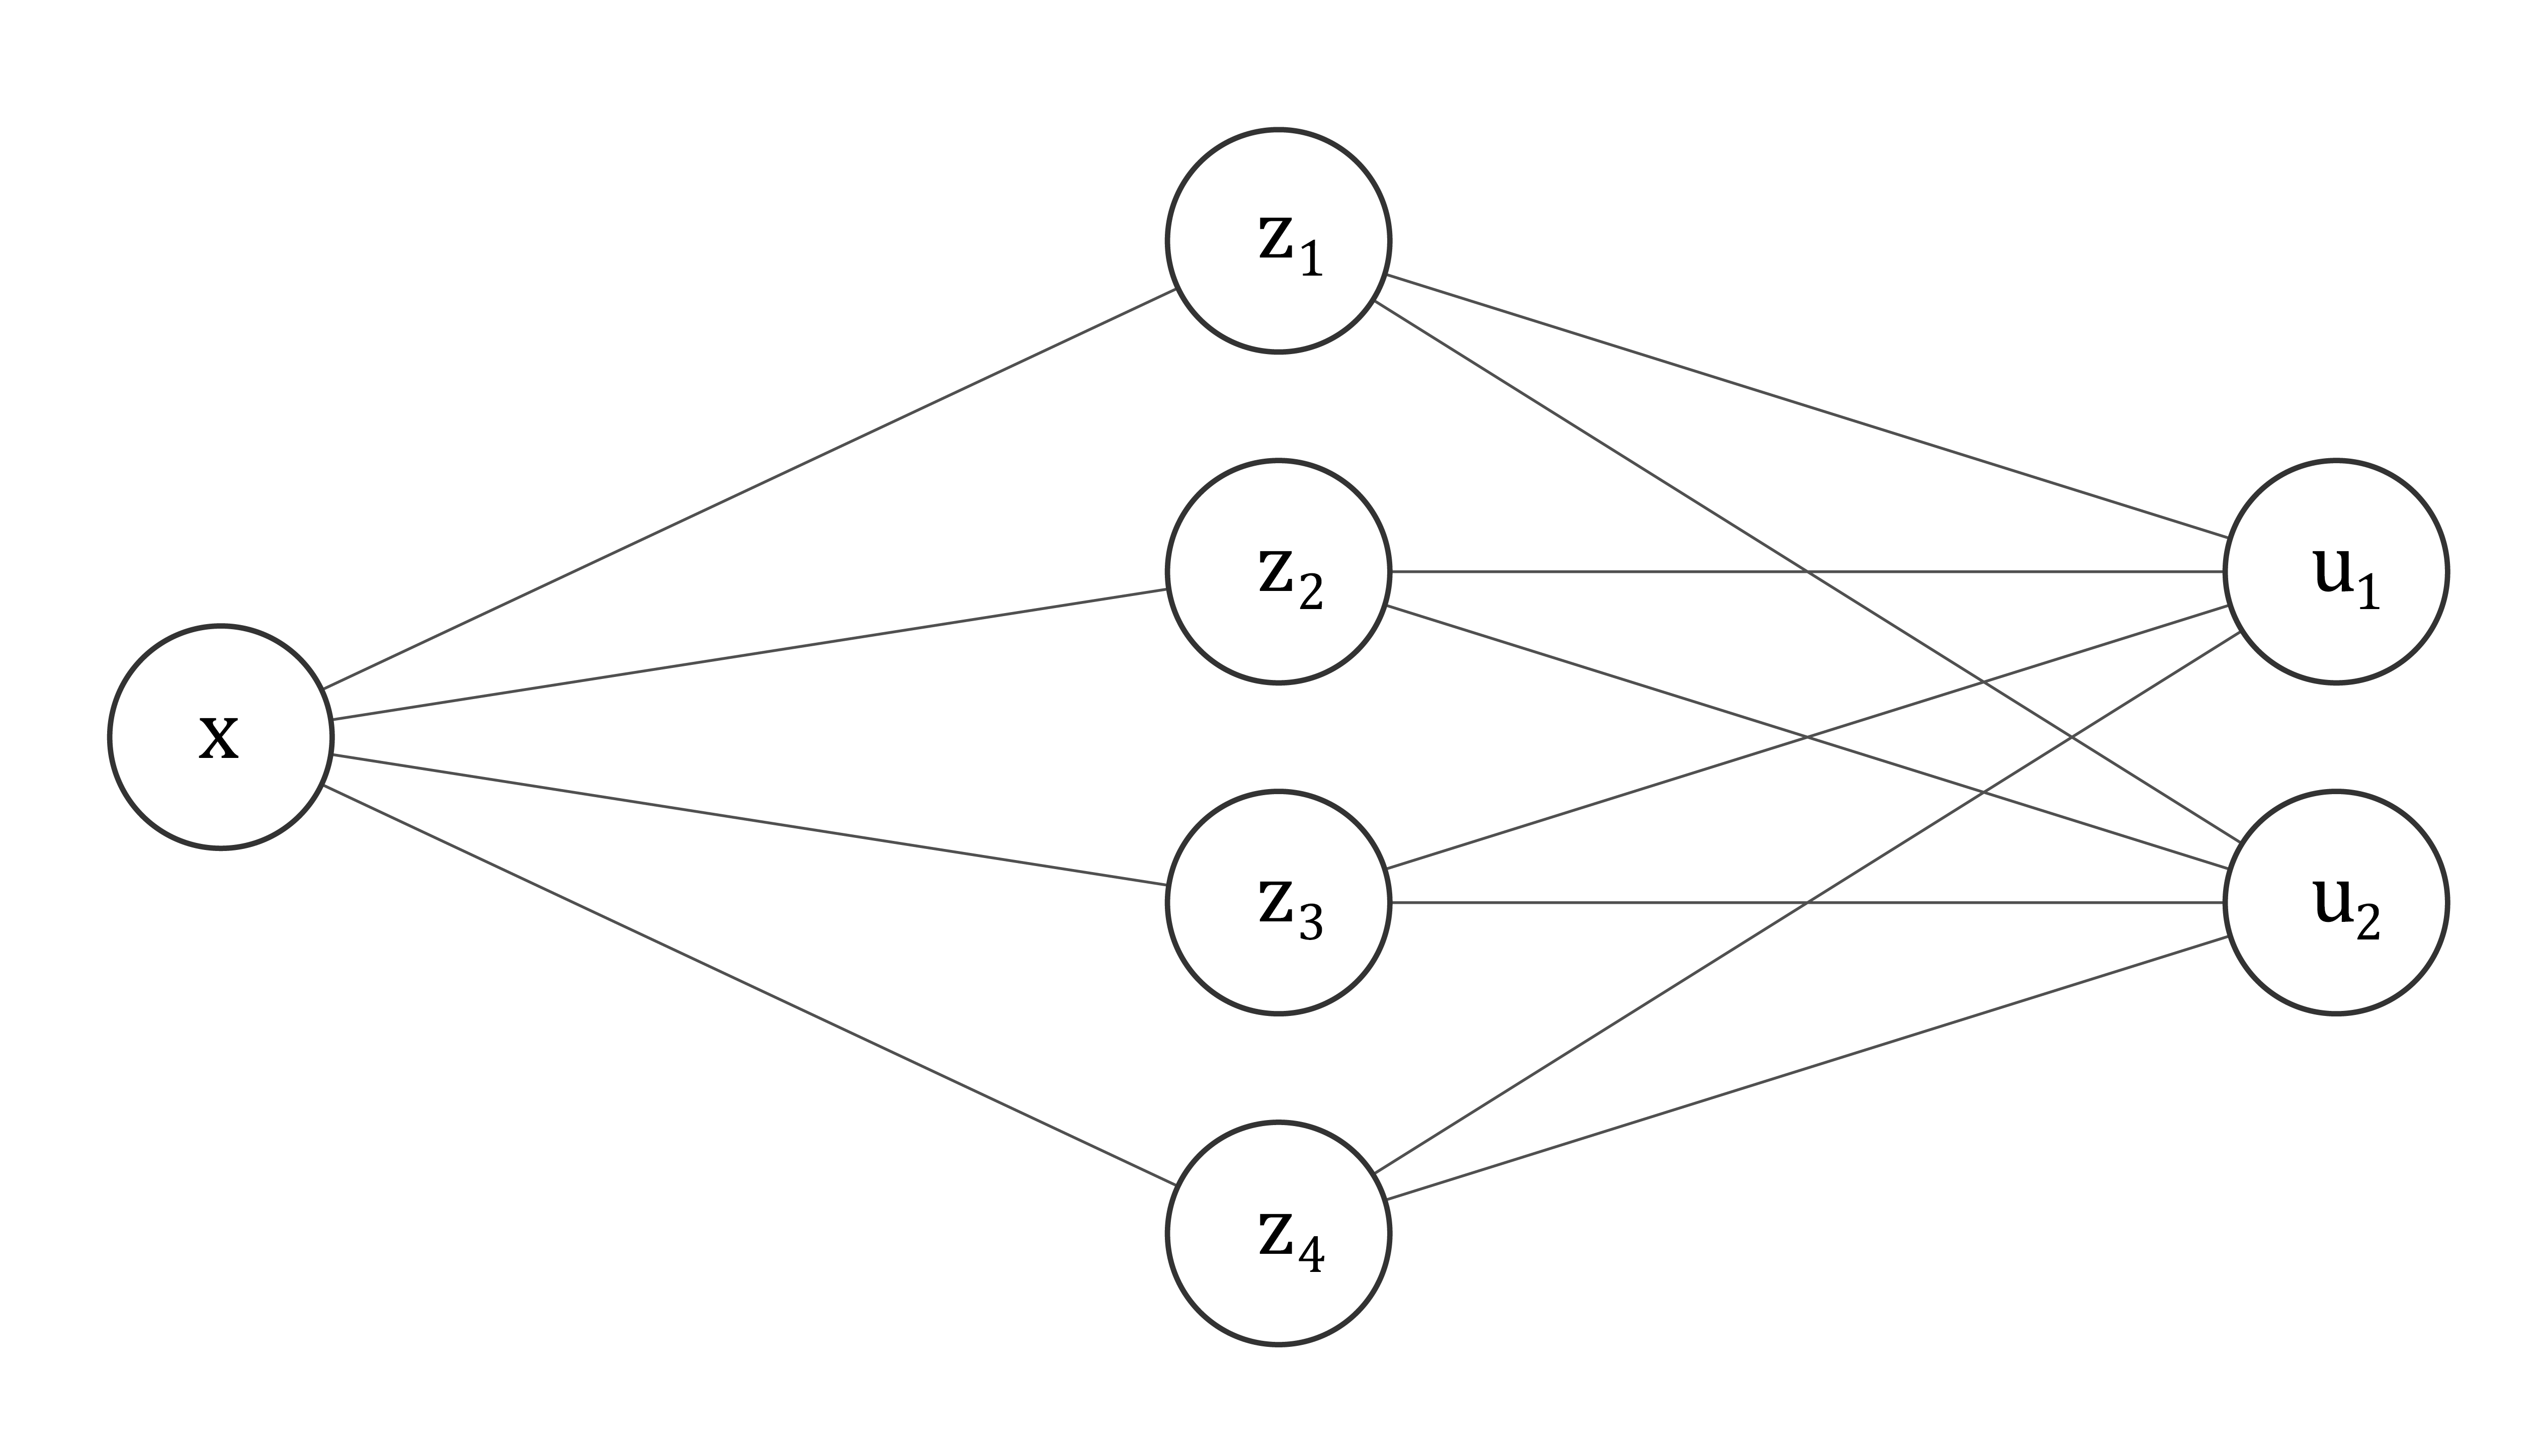
\includegraphics[width=\textwidth]{img/ShallowMLP.png}
        \caption{Shallow multilayer perceptron with $N=3$.}
        \label{fig:vpinnshallowmlp}
    \end{subfigure}
\end{figure}

With this structure, the network has $2N$ parameters for the first hidden layer, $(D-1)(N^2+N)$ parameters for other hidden layers, and $2N+2$ parameters for the last year, which sums up as
\begin{equation}
    \label{eq:vpinnsparameters}
    N_p = (D-1)N^2+(D+3)N+2,
\end{equation}
where $N_p$ is total number of parameters of the network.

\subsubsection{Basis representation}\label{sec:vpinnsbasis}
% TODO: Elaborate on the linear combination of the basis at the last layer, show shallow network formulation with ReLU

\subsubsection{Variational formulation for VPINNs}\label{sec:vpinnsformulation}
Let $V_K = span(v_1, v_2, \cdots, v_K)$ be the space of the test functions. The helmholtz impedance problem in the context of VPINNs is defined as finding $u_{\mathcal{N}} \in \mathcal{N}$ such that the loss function
\begin{equation}
    \label{eq:lossfunction}
    \mathcal{L}^2(u_{\mathcal{N}}) = \frac{1}{K} \sum_{k=1}^{K}{|R_k^{(2)} - F_k|^2}
\end{equation}
is minimized, where
\begin{equation}
    \label{eq:vpinnrhs}
    R_k^{(2)} = \int_{a}^{b}{u'_{\mathcal{N}}v'_k} - k^2 \int_{a}^{b}{u_{\mathcal{N}}v_k} - (g_a + \imath ku_{\mathcal{N}}(a))v_k(a) - (g_b + \imath ku_{\mathcal{N}}(b))v_k(b),
\end{equation}
\begin{equation}
    \label{eq:vpinnlhs}
    F_k = \int_{a}^{b}{fv_k}.
\end{equation}

\subsubsection{Morawetz- and Rellich-Type Identities}\label{sec:vpinnsformulationhq}
% TODO: Why this formulation? Makes it elliptic or makes the matrix spd?
Another variational formulation of the Helmholtz impedance problem is presented and analyzed in \cite{moiola2014helmholtz}. A modification of this formulation for the one dimensional case is provided in \cite{henriquez2022}, which is presented in this subsection. Let $u, v \in L^2(\Omega)$ and consider $\Omega=[-1,+1]$. For $k, \beta \in \mathbb{R}$, set $\mathcal{L}v= v''+k^2v$ and define
\begin{equation}
    \mathcal{M}v=xv'-\imath k \beta v.
\end{equation}
Consider the sesquilinear form $a:H^2(\Omega)\times H^2(\Omega) \to \mathbb{C}$ defined as
\begin{equation}
    \begin{split}
        a(u, v) & := \int_{\Omega}{u'\bar{v}'} + k^2 \int_{\Omega}{u\bar{v}} + \int_{\Omega} \left ( \mathcal{M}u + \frac{A}{k^2}\mathcal{L}u\right )\overline{\mathcal{L}v} \\ & - \imath k (\overline{\mathcal{M}v(b)}u(b) + \overline{\mathcal{M}v(a)}u(a)) - \bar{v}'\mathcal{M}u|_{\partial \Omega} - xk^2u\bar{v}|_{\partial \Omega} + xu'\bar{v}'|_{\partial \Omega}
    \end{split}
\end{equation}
and the linear form $b:H^2(\Omega) \to \mathbb{C}$ defined as
\begin{equation}
    b(v) := \int_{\Omega}{\left ( \overline{\mathcal{M}v} - \frac{A}{k^2} \overline{\mathcal{L}v} \right )f + \overline{\mathcal{M}v(b)}g_b + \overline{\mathcal{M}v(a)}g_a},
\end{equation}
where $A>0 \in \mathbb{R}$. The problem would be defined as finding $u \in H^2(\Omega)$ such that $a(u,v)=b(v)$ for all $v \in H^2(\Omega)$. As suggested in \cite{henriquez2022}, setting $\beta = 1$ and $A = 1/3$ makes the sesquilinear form $a$ V-elliptic.

\subsubsection{Least Squares Initialization}\label{sec:lsinit}


\subsubsection{Quadrature rules for integrations}\label{sec:quadraturerules}
% TODO: Explain the local and global quadrature points
% TODO: Mention quadrature methods

\section{Results And Discussion}\label{sec:results}
The results of each method are presented and discussed in this section. We define the error of the solution as the $H^1{(\Omega)}$ norm of difference between the analytical solution $u(x)$, and the solution of the numerical scheme $u_N(x)$ as
\begin{equation}
    \label{eq:H1error}
    ||u(x) - u_N(x)||_{H^1{(\Omega)}} = ||u(x) - u_N(x)||_{L^2{(\Omega)}} + ||u'(x) - u'_N(x)||_{L^2{(\Omega)}},
\end{equation}
where
\begin{equation}
    \label{eq:L2error}
    ||f(x)||_{L^2{(\Omega)}} = \begin{pmatrix} \int_{\Omega}{|f(x)|^2dx} \end{pmatrix}^{1/2},
\end{equation}
and use this error as a measure to evaluate the solution from each numerical scheme.

\subsection{Finite elements scheme}\label{sec:femresults}
Implementing the framework described in \autoref{sec:femframework}, we investigated the results of the finite element scheme for the Helmholtz impedance problem with different frequencies. The results for a relatively moderate $k$ validated against the exact solution are presented in Figures \ref{fig:femMidfreqN050} and \ref{fig:femMidfreqN100}. These plots show how using a finer mesh (bigger $N$) on the domain improves the quality of the solution. The same trend has been observed for other $k$'s.

\begin{figure}[h!]
    \centering
    \begin{subfigure}[b]{0.7\textwidth}
        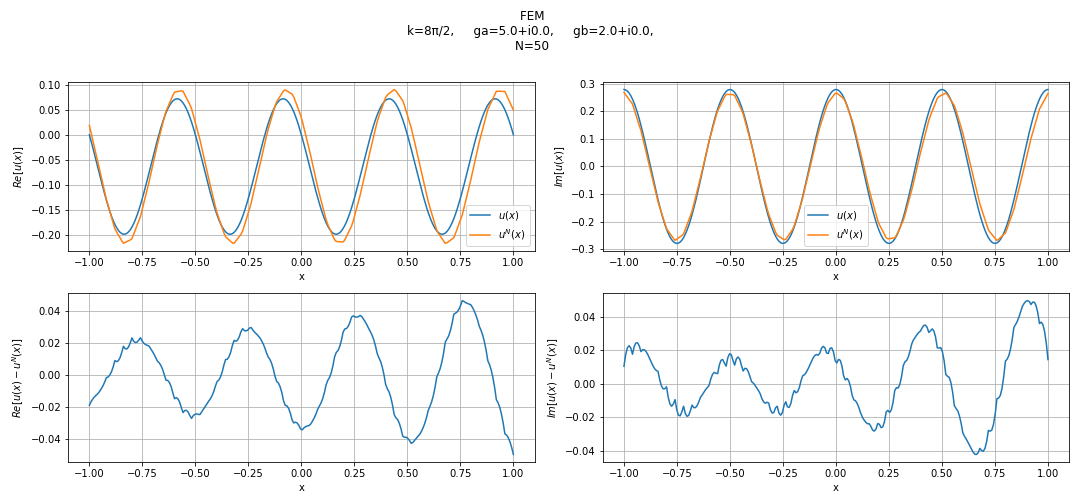
\includegraphics[width=\textwidth]{img/FEM-Const-MidFreq-N0050-sol.png}
        \caption{$u_N(x)$}
    \end{subfigure}
    \vfill
    \begin{subfigure}[b]{0.7\textwidth}
        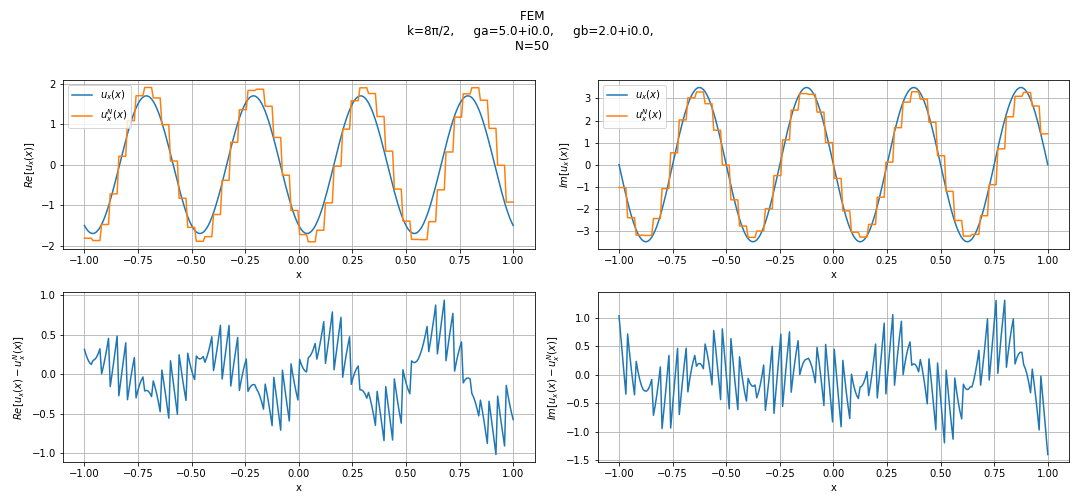
\includegraphics[width=\textwidth]{img/FEM-Const-MidFreq-N0050-der.png}
        \caption{$u'_N(x)$}
    \end{subfigure}
    \caption{$u_N(x)$ (a) and $u'_N(x)$ (b) plotted against the exact solution for a relatively moderate $k$ and $N=50$. On each subfigure, the bottom row represents the difference between the numerical and exact solutions. The source function has a constant value of $f(x)=10$, and other parameters are indicated on the figures.}
    \label{fig:femMidfreqN050}
\end{figure}
\begin{figure}[h!]
    \centering
    \begin{subfigure}[b]{0.7\textwidth}
        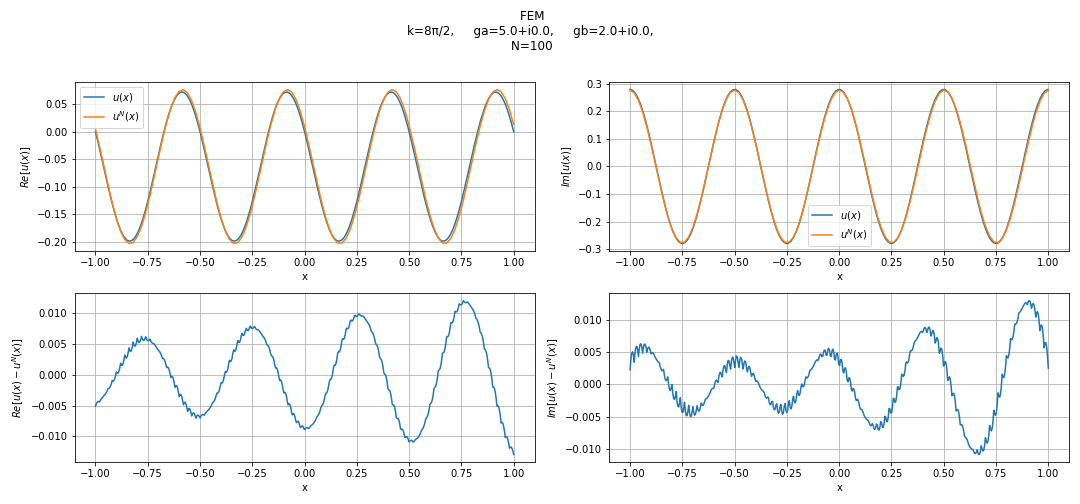
\includegraphics[width=\textwidth]{img/FEM-Const-MidFreq-N0100-sol.png}
        \caption{$u_N(x)$}
    \end{subfigure}
    \vfill
    \begin{subfigure}[b]{0.7\textwidth}
        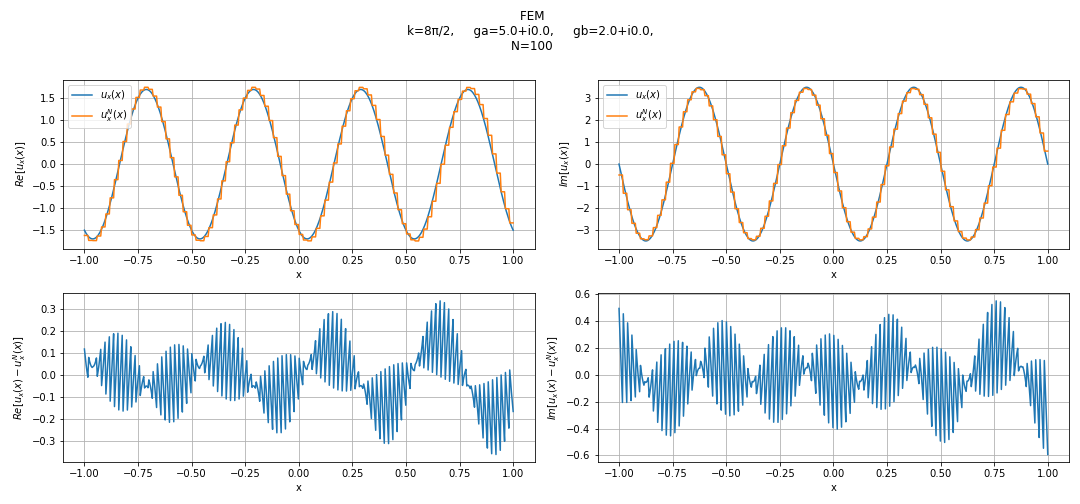
\includegraphics[width=\textwidth]{img/FEM-Const-MidFreq-N0100-der.png}
        \caption{$u'_N(x)$}
    \end{subfigure}
    \caption{$u_N(x)$ (a) and $u'_N(x)$ (b) plotted against the exact solution for a relatively moderate $k$ and $N=100$. On each subfigure, the bottom row represents the difference between the numerical and exact solutions. The source function has a constant value of $f(x)=10$, and other parameters are indicated on the figures.}
    \label{fig:femMidfreqN100}
\end{figure}

However, for larger values of $k$, there is an issue with this method. From the nature of the equation we know that for larger $k$'s, we have more oscillations in the solution. Since our FEM is estimating the solution with piecewise linear basis functions in a uniform mesh, the resulting numerical solution will also be piecewise linear. This will require a minimum number of grid points on each oscillation for the estimation to have a decent accuracy. Consider the solution in \autoref{fig:femMidfreqN100} where we used 100 grid points. If we wanted to estimate this function with 8 grid points, for instance, it was not possible to even capture the general shape of the function. This phenomenon is the major observation in \autoref{fig:femorder}, where the H1-error of the numerical solution is plotted against mesh refinement parameter, $N$, for different values of $k$. For each constant $k$, there is no improvement in the error as we refine the mesh until a certain $N$, which will be called $N_c$ in the rest of this report. However, for $N > N_c$, we can see the first order accuracy of the method as we expected. Another important observation is that the value of $N_c$ increases with increasing $k$, which means that for high values of $k$, the improvement in the accuracy only begins at a very high $N$.
\begin{figure}[h!]
    \centering
    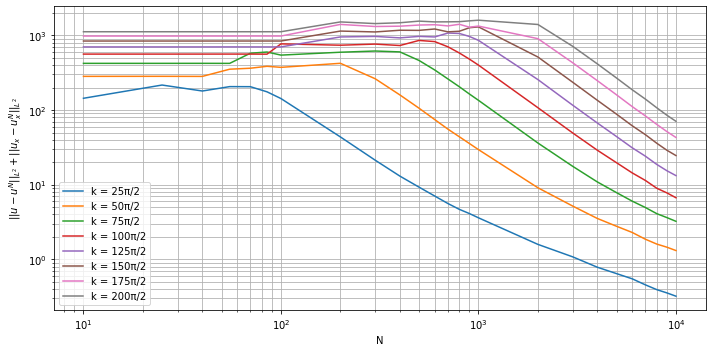
\includegraphics[width=.7\textwidth]{img/FEM-Order-Homog-H1.png}
    \caption{Order of accuracy of the FEM scheme for different values of $k$.}
    \label{fig:femorder}
    % TODO: Add the -1 slope to the plot.S
\end{figure}

\subsection{VPINNs Scheme}\label{sec:vpinnsresults}
Implementing the framework explained in \autoref{sec:vpinnsframework}, we investigated the performace of this scheme for different network structures, different activation functions, different training methods, and for different frequencies $k$. The Adam optimizer~\cite{adamoptimizer} is used for all trainings. The weights of each layer are initialized using the normal Xavier initialization~\cite{xavierinitialization}, and the biases are initialized using a uniform distribution in the domain $\Omega$. Each training is done multiple times to ensure independance from randomness and the best one is selected for comparisons. On each set of the trainings, the biggest possible learning rate $lr$ that ensures convergence for all the networks being compared is selected.

\subsubsection{Shallow Networks}

\begin{figure}[h!]
    \centering
    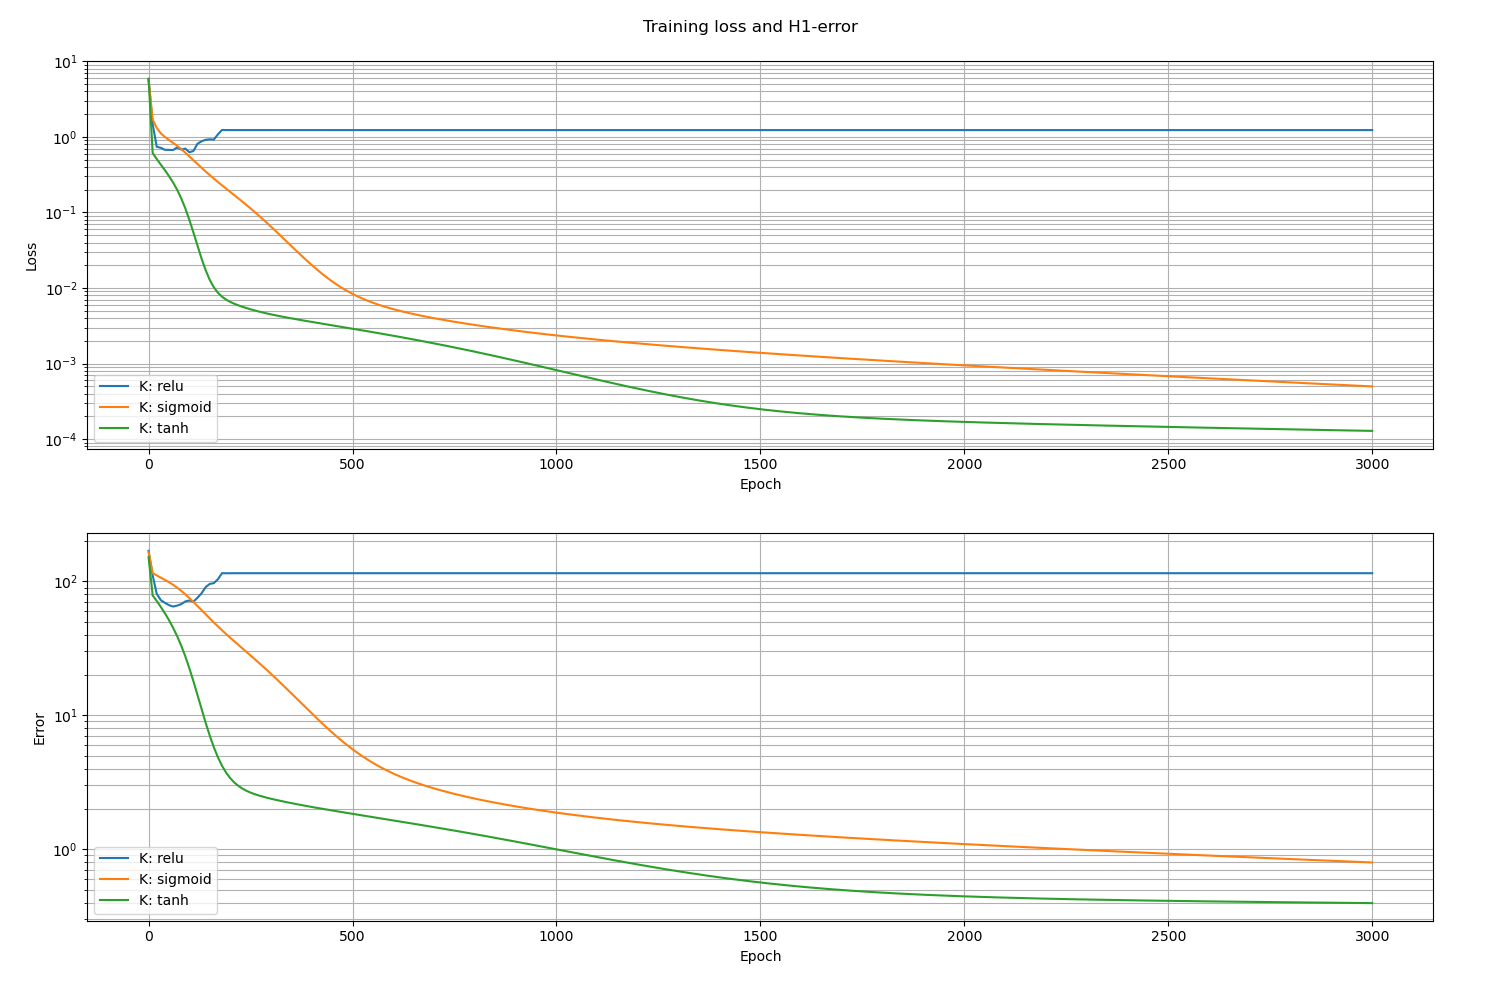
\includegraphics[width=.7\textwidth]{img/VPINN-Comparison-Activation.png}
    \caption{Training loss and H1-error of a shallow network with $N=10$ and $K=10$ with different activation functions for $k=1.0$.}
    \label{fig:activationfunctions}
\end{figure}

We start with shallow neural networks with only one hidden layer, i.e. $D=1$. We use the local hat functions presented in \autoref{eq:fembasisfuncs} as test functions, and train a network with $N=10$ and 10 test functions ($K=10$) with different types of activation functions for a low frequency. The loss functions and the errors are compared in \autoref{fig:activationfunctions}. The learning rate is $1E{-01}$ for all the activation functions. We can see that the hyperbolic tangent activation function outperforms the sigmoid activation function for our setup both in terms of accuracy and convergence rate. Regarding the ReLU activation function, there are some issues inherited with this set-up of networks. If we train the weights and biases of the hidden layer, these parameters drive the threshold of each ReLU outside of the support domain of the test functions, and the gradient of the loss with respect to these parameters go to zero, so technically, the hidden neurons will be lost one by one. As done in \cite{liu2021}, it could be easily shown that in case of the ReLU activation function, the weights of the hidden layer are redundent for this kind of networks and it is suggested to set the weights to 1. To address the issue with ReLU activation function, the network is trained with fixed biases being uniformly distributed in the domain $[a, b]$ and weights fixed to 1, and the training could be completed withough this issue. However, by fixing the parameters of the hidden layer and the ReLU activation function, this framework has no advantage over the original FEM scheme in case of capability and adaptability. In the rest of the experiments, the hyperbolic tangent activation function is used for the trainings.

\begin{figure}[h!]
    \centering
    \begin{subfigure}[b]{0.48\textwidth}
        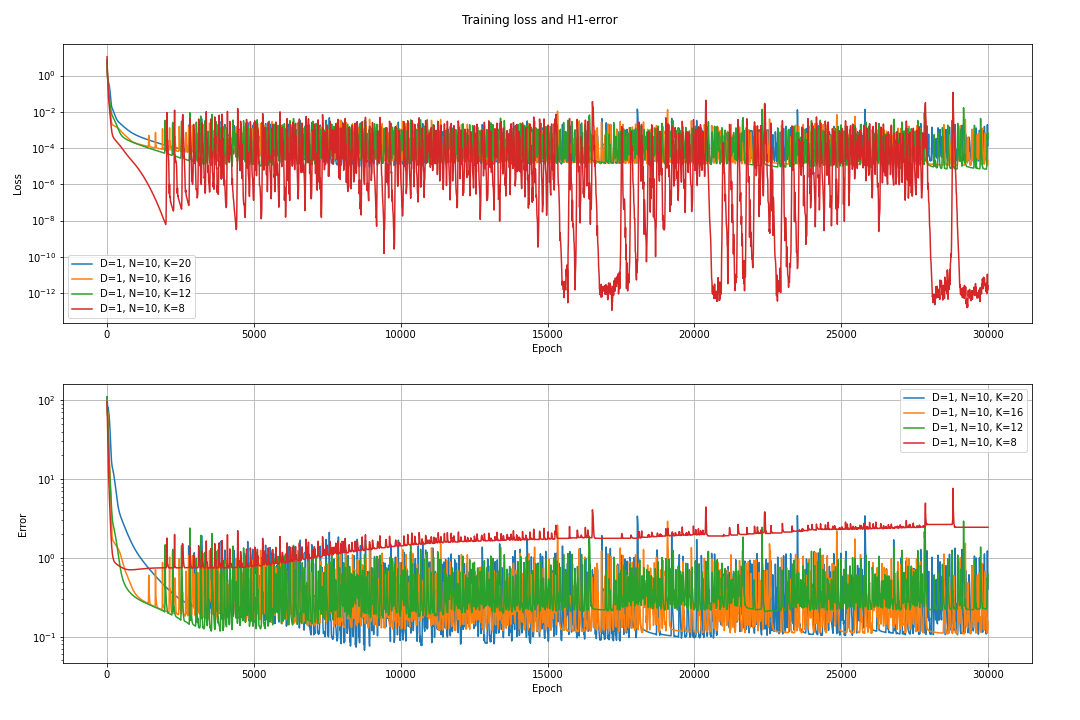
\includegraphics[width=\textwidth]{img/VPINN-Comparison-k2increaseK.png}
        \caption{$k=2$.}
        \label{fig:vpinnsk2increaseK}
    \end{subfigure}
    \hfill
    \begin{subfigure}[b]{0.48\textwidth}
        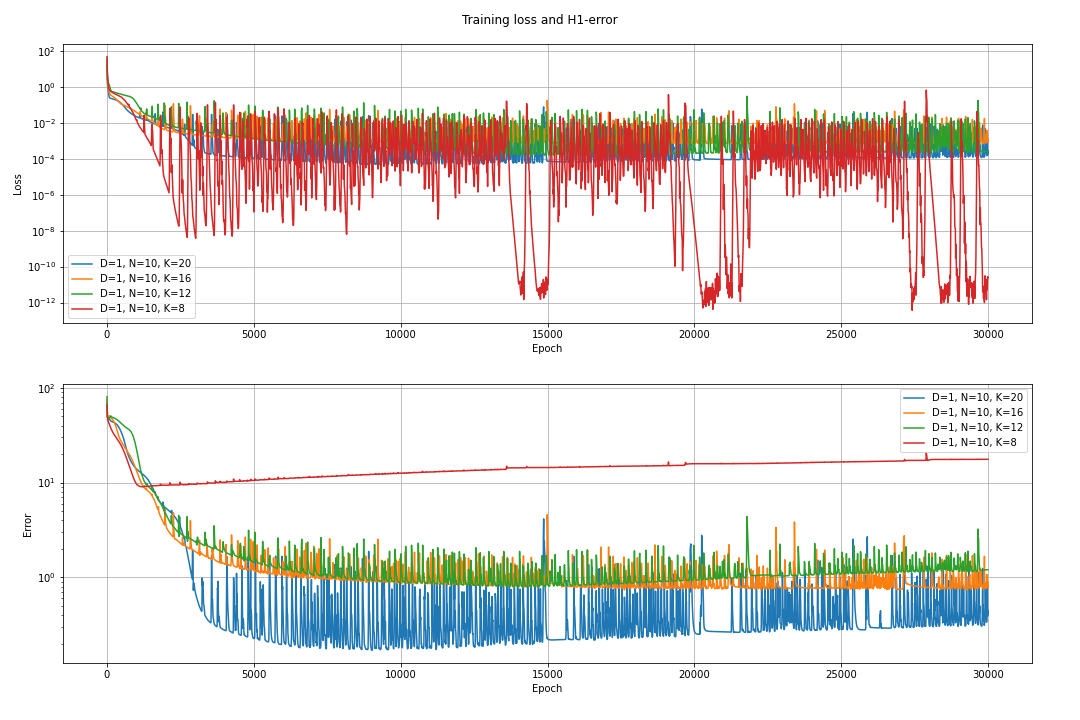
\includegraphics[width=\textwidth]{img/VPINN-Comparison-k4increaseK.png}
        \caption{$k=4$.}
        \label{fig:vpinnsk4increaseK}
    \end{subfigure}
    \vfill
    \begin{subfigure}[b]{0.48\textwidth}
        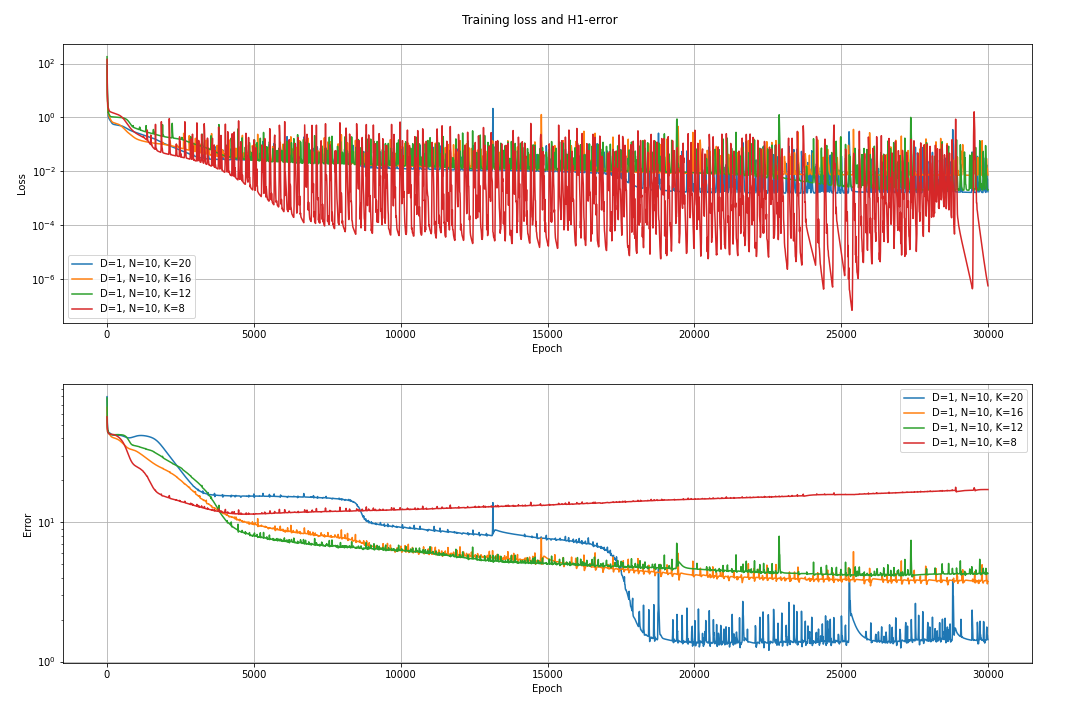
\includegraphics[width=\textwidth]{img/VPINN-Comparison-k6increaseK.png}
        \caption{$k=6$.}
        \label{fig:vpinnsk6increaseK}
    \end{subfigure}
    \hfill
    \begin{subfigure}[b]{0.48\textwidth}
        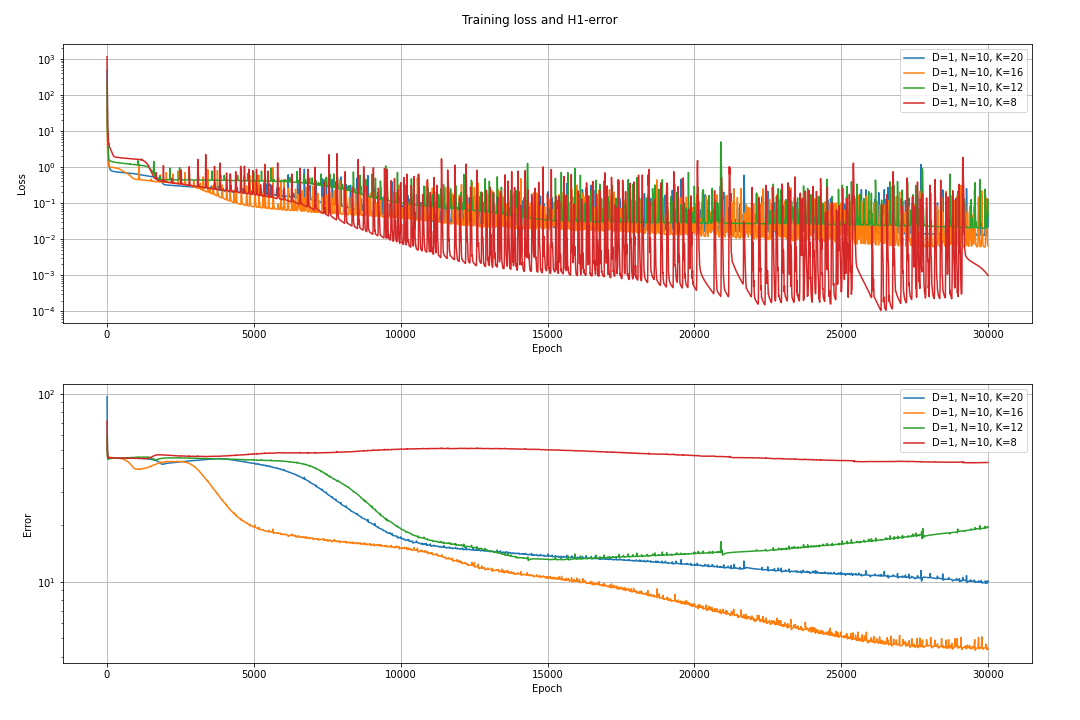
\includegraphics[width=\textwidth]{img/VPINN-Comparison-k8increaseK.png}
        \caption{$k=8$.}
        \label{fig:vpinnsk8increaseK}
    \end{subfigure}
    \caption{Training loss and H1-error with fixed network structure and increasing number of test functions for different frequencies.}
    \label{fig:vpinnsincreaseK}
\end{figure}

In an effort to investigate the effect of increasing the number of test functions on the accuracy and the training of the network, with a fixed width $N=10$, the training is done for different values of $K$. The results are presented in \autoref{fig:vpinnsincreaseK}. For the lowest frequency $k=2$ in \autoref{fig:vpinnsk2increaseK}, we can see that with 8 test functions, the training loss becomes unstable and the H1-error takes an increasing trend after around 2000 epochs. With 12 test functions, this behavior is not observed and the H1-error converges. Increasing the number of test functions to 16, we can see a slight improvement, which does not repeat with further increasing the number of test functions to 20. For a higher frequency $k=4$ in \autoref{fig:vpinnsk4increaseK}, we can see the same behavior for 8 test functions but with the difference that the final H1-error keeps being improved with increasing the number of test functions to 20. For the highest frequency $k=8$, we can observe the unstable behavior extends to 12 test functions, and the improvement with increasing the number of test functions becomes more evident. We can conclude that as the frequency increases, more number of test functions will be needed for training the network.

\begin{figure}[h!]
    \centering
    \begin{subfigure}[b]{0.48\textwidth}
        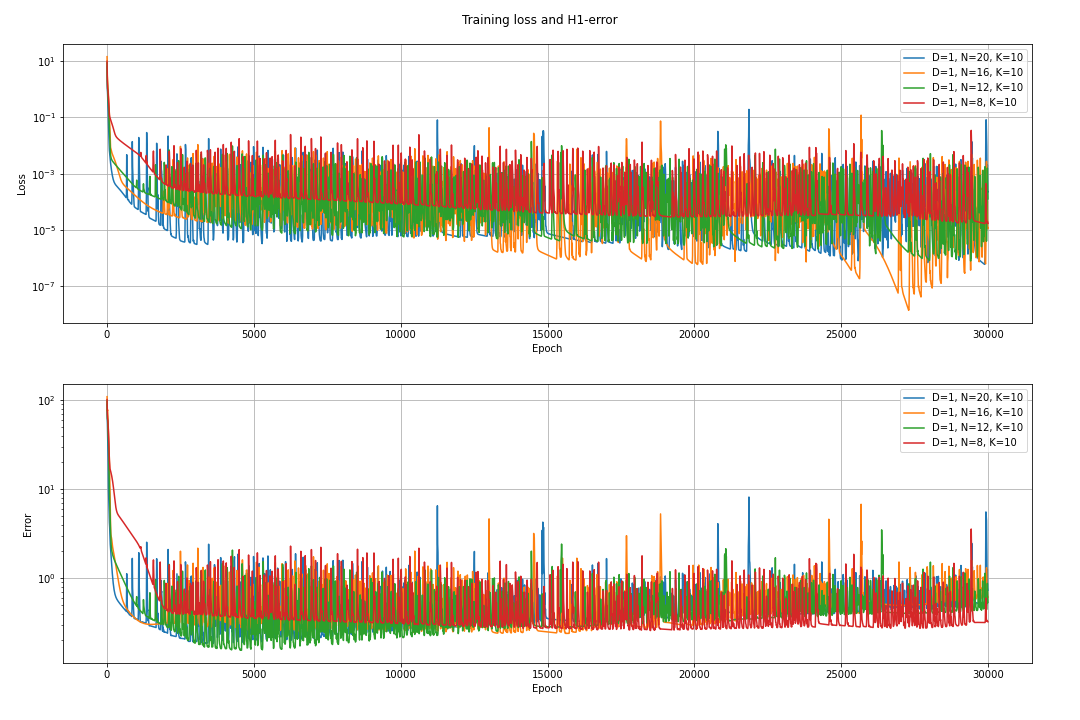
\includegraphics[width=\textwidth]{img/VPINN-Comparison-k2increaseN.png}
        \caption{$k=2$.}
        \label{fig:vpinnsk2increaseN}
    \end{subfigure}
    \hfill
    \begin{subfigure}[b]{0.48\textwidth}
        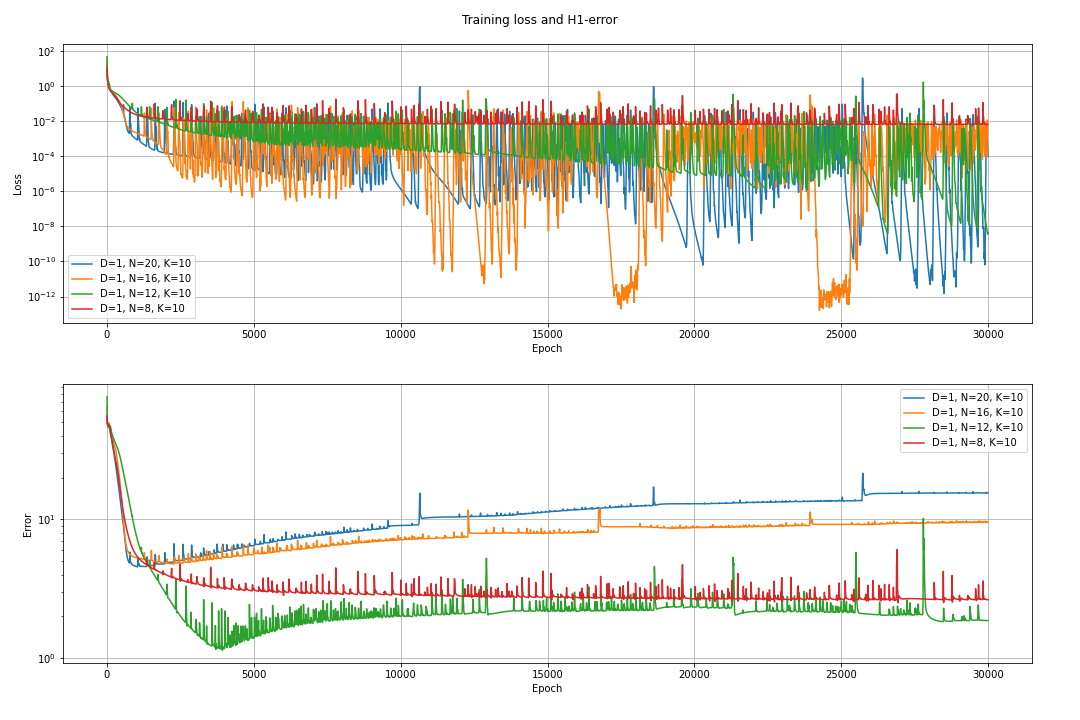
\includegraphics[width=\textwidth]{img/VPINN-Comparison-k4increaseN.png}
        \caption{$k=4$.}
        \label{fig:vpinnsk4increaseN}
    \end{subfigure}
    \vfill
    \begin{subfigure}[b]{0.48\textwidth}
        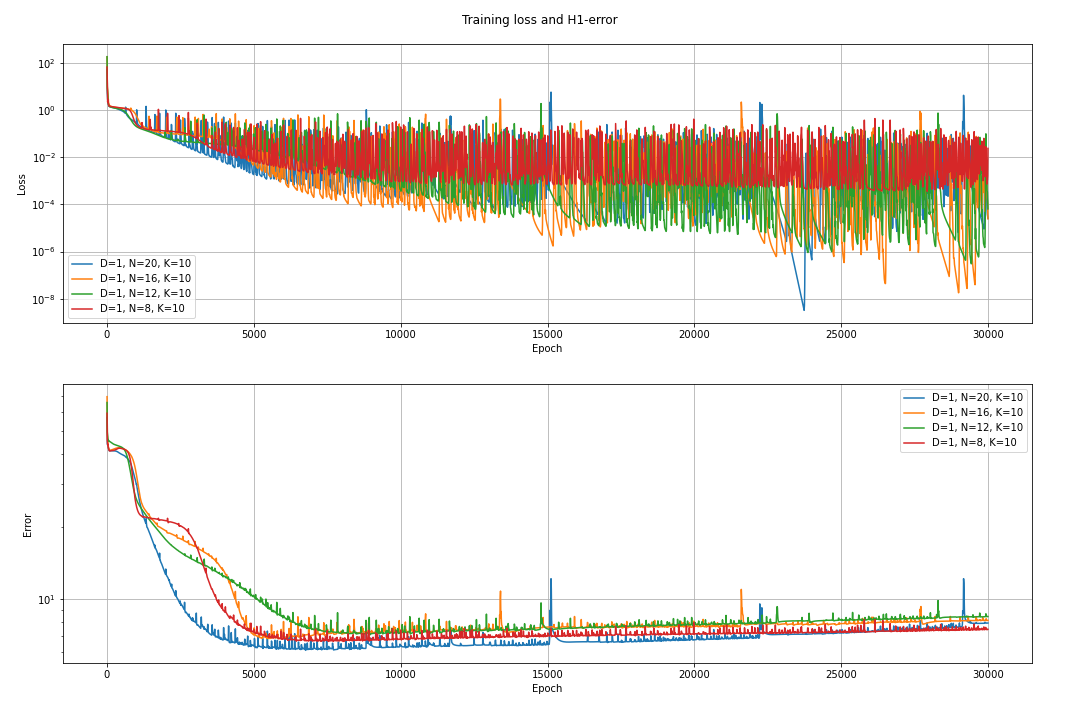
\includegraphics[width=\textwidth]{img/VPINN-Comparison-k6increaseN.png}
        \caption{$k=6$.}
        \label{fig:vpinnsk6increaseN}
    \end{subfigure}
    \hfill
    \begin{subfigure}[b]{0.48\textwidth}
        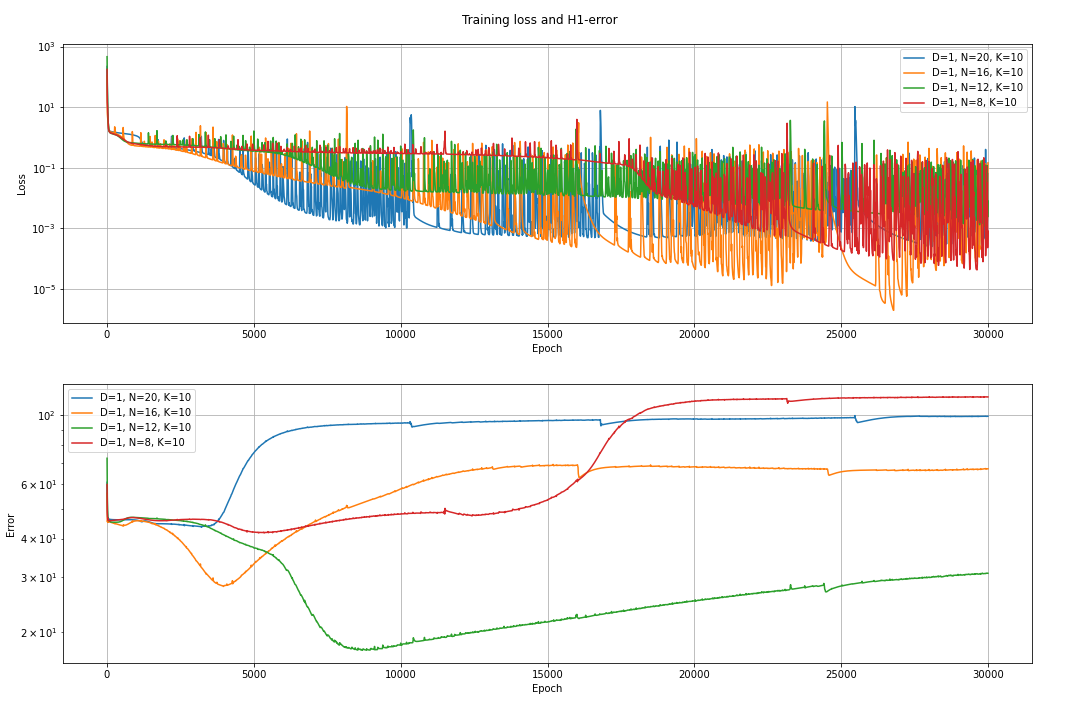
\includegraphics[width=\textwidth]{img/VPINN-Comparison-k8increaseN.png}
        \caption{$k=8$.}
        \label{fig:vpinnsk8increaseN}
    \end{subfigure}
    \caption{Training loss and H1-error with fixed number of test function and increasing width of the network.}
    \label{fig:vpinnsincreaseN}
\end{figure}

To investigate the effect of the width of the network, a similar thing is done with fixing the number of test functions to $K=10$, and training the network for different values of $N$. The results are presented in \autoref{fig:vpinnsincreaseN}. For the lowest frequency $k=2$ in \autoref{fig:vpinnsk2increaseN}, we can see that increasing the width of the network does not bring much to the table. However, the network reaches its minimum H1-error faster. For $k=4$ in \autoref{fig:vpinnsk4increaseN}, we can see that when the width of the network is increased to $16$ or $20$, the unstable behavior emerges even for sufficient number of test functions. For higher frequencies, the network is not able to converge to the solution with any of these widths, and we can see that increasing the width even makes things worse in \autoref{fig:vpinnsk8increaseN}. These obseervations allows to conclude that increasing the width of the network cannot heal the need for higher number of test functions, and even require more number of test functions in order to converge to the solution.

\begin{figure}[h!]
    \centering
    \begin{subfigure}[b]{0.48\textwidth}
        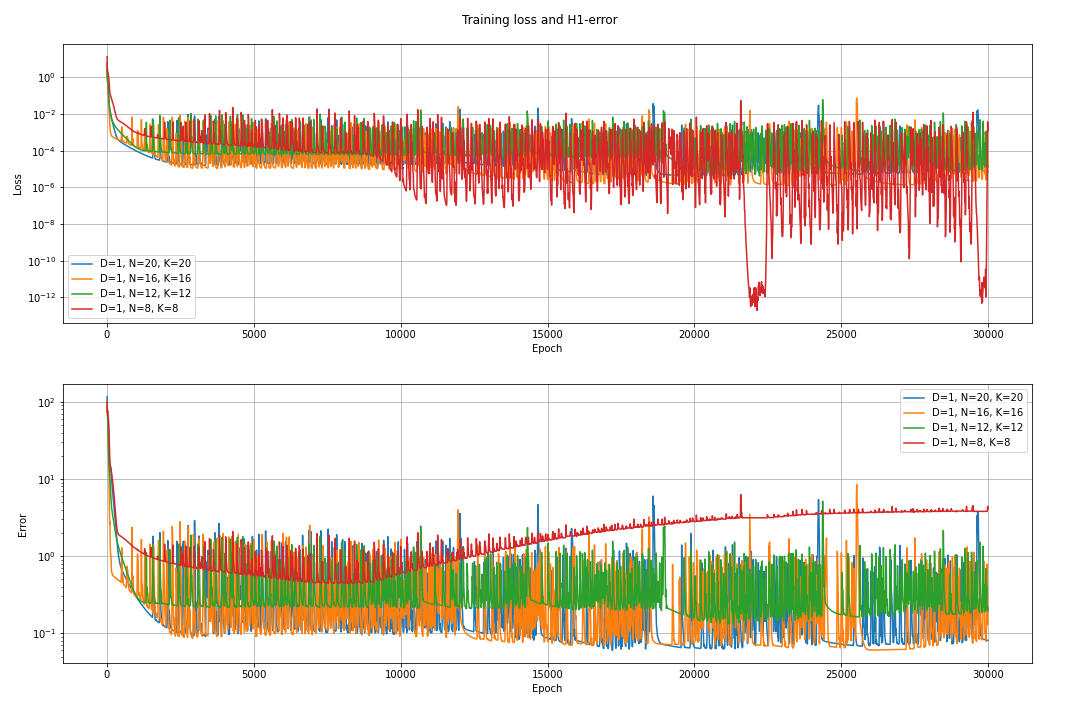
\includegraphics[width=\textwidth]{img/VPINN-Comparison-k2increaseNK.png}
        \caption{$k=2$.}
        \label{fig:vpinnsk2increaseNK}
    \end{subfigure}
    \hfill
    \begin{subfigure}[b]{0.48\textwidth}
        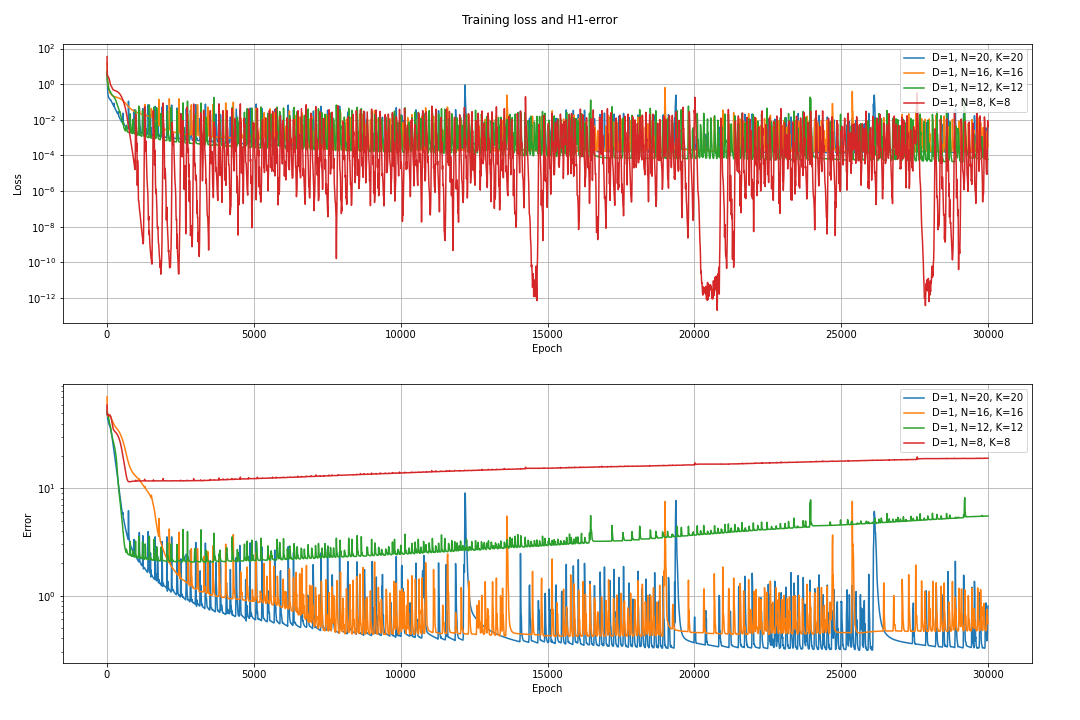
\includegraphics[width=\textwidth]{img/VPINN-Comparison-k4increaseNK.png}
        \caption{$k=4$.}
        \label{fig:vpinnsk4increaseNK}
    \end{subfigure}
    \vfill
    \begin{subfigure}[b]{0.48\textwidth}
        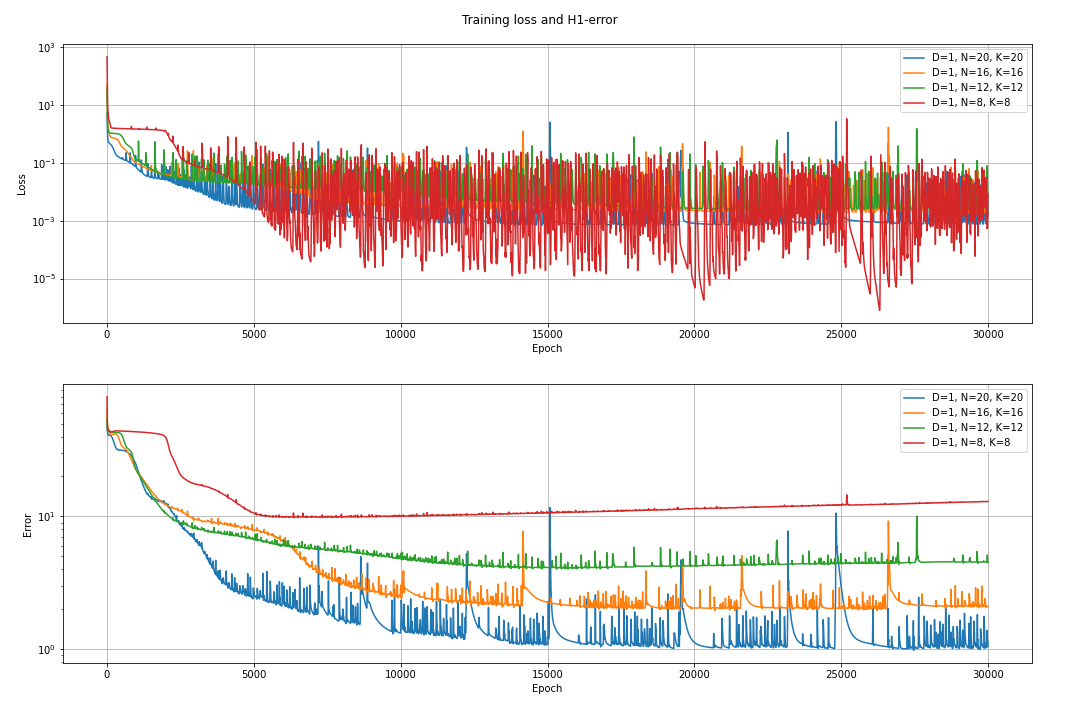
\includegraphics[width=\textwidth]{img/VPINN-Comparison-k6increaseNK.png}
        \caption{$k=6$.}
        \label{fig:vpinnsk6increaseNK}
    \end{subfigure}
    \hfill
    \begin{subfigure}[b]{0.48\textwidth}
        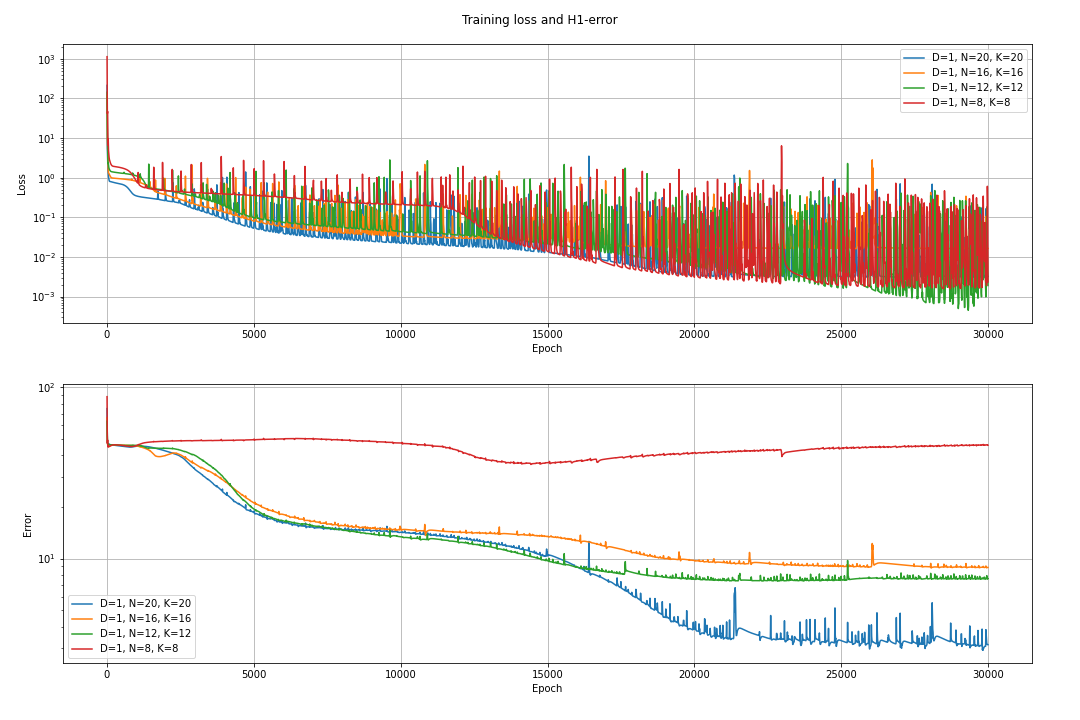
\includegraphics[width=\textwidth]{img/VPINN-Comparison-k8increaseNK.png}
        \caption{$k=8$.}
        \label{fig:vpinnsk8increaseNK}
    \end{subfigure}
    \caption{Training loss and H1-error with fixed number of test function and increasing width of the network.}
    \label{fig:vpinnsincreaseNK}
\end{figure}

In another set of experiments, the width of the network and the number of test functions are kept equal and are increased together. The idea was to treat these two hypermarameters as one parameter since they are bounded together in FEM. The results are presented in \autoref{fig:vpinnsincreaseNK}. We can see that the final H1-error is consistently improved with increasing both $N$ and $K$ together for all of the frequencies, but the improvement becomes more evident as the frequency gets higher. These experiments confirm that the best approach is to keep $N$ and $K$ proportional, and increase them together in order to study the convergence rate of this method.
% TODO: Conclusion: N correlated to K is the best, increase them together, maybe for specific problems the ratio between these two could be optimized.

\begin{figure}[h!]
    \centering
    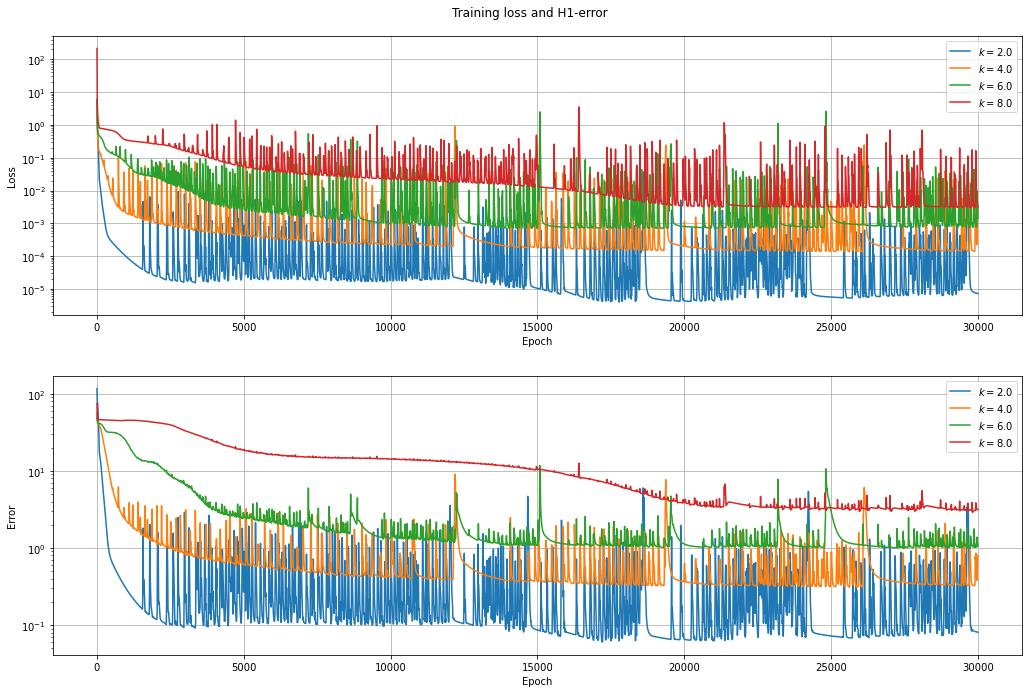
\includegraphics[width=.7\textwidth]{img/VPINN-Comparison-NK20increasek.png}
    \caption{Training loss and H1-error of a shallow network with $N=20$ and $K=20$ for different frequencies.}
    \label{fig:vpinnsincreasefreq}
\end{figure}

Figure \ref{fig:vpinnsincreasefreq} shows how a quite strong network with $N=K=20$ performs for different frequencies. Although the network is doing a good job for all of the frequencies, we can see that as the frequency increases, the accuracy of the final solution decreases, which again implies the need to enrich the network for higher frequencies.

\subsubsection{Deep Networks}\label{seq:deepnetworks}
From \autoref{eq:vpinnsparameters}, we can see that for deeper neural networks ($D>1$), the number of parameters has a quadratic dependancy on the width of the network, $N$. This gave us the notion that just as increasing $N$ would require more test functions, increasing $D$ might also require the training to be done on more test functions. To address this, we compared the training process for a network with two hidden layers and $N=12$ with different number of test functions. The results are presented in \autoref{fig:vpinnsdeepincreaseK}. We can see that with the same number of test functions as for shallow networks, the model is overfitted to the test functions. While with 20 test functions we can get a better H1-error, further increasing the number of test functions to 28 is not advantageous. We conclude that 24 test functions as adequate for this network structure with 206 parameters. Comparing this number to the number of parameters (50) of the shallow network with the same width, we can assume that the number of adequate test functions scales with the square root of the number of parameters: $K_{adequate} \sim \sqrt{N_p}$.
% TODO: Conclusion: The number of adequate test functions is proportional to the square root of the number of parameters.

\begin{figure}[h!]
    \centering
    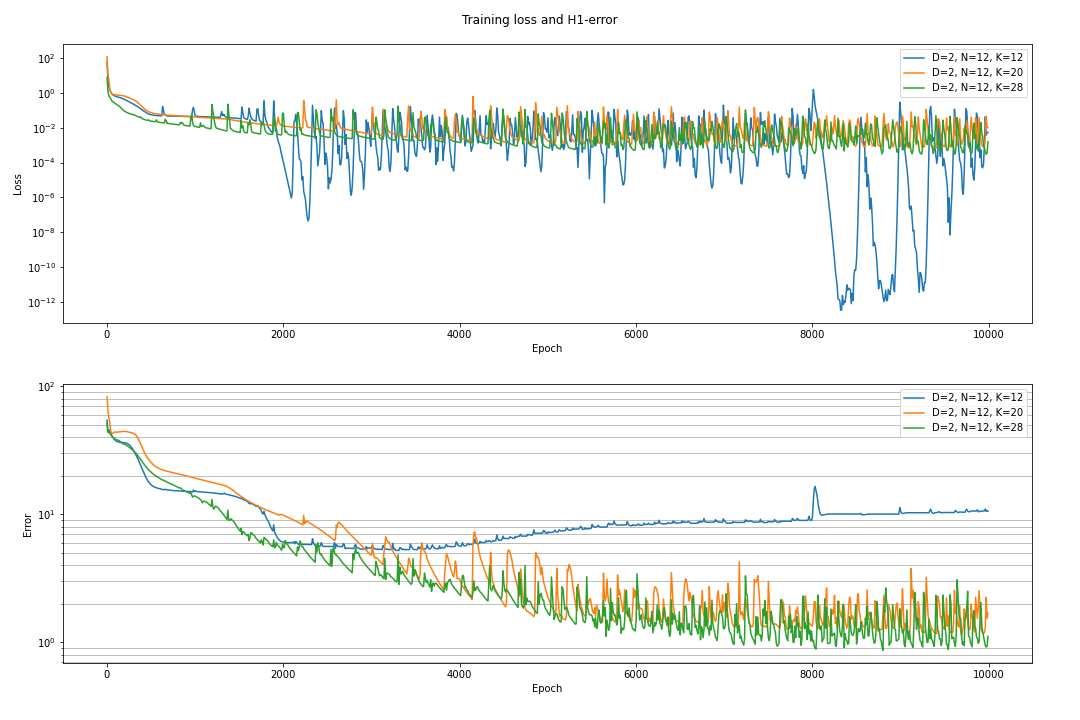
\includegraphics[width=.7\textwidth]{img/VPINN-Deep-Comparison-k8increaseK.png}
    \caption{Training loss and H1-error of a network with 2 hidden layers and $N=12$ for frequency $k=8.0$, with different number of test functions.}
    \label{fig:vpinnsdeepincreaseK}
\end{figure}

\begin{figure}[h!]
    \centering
    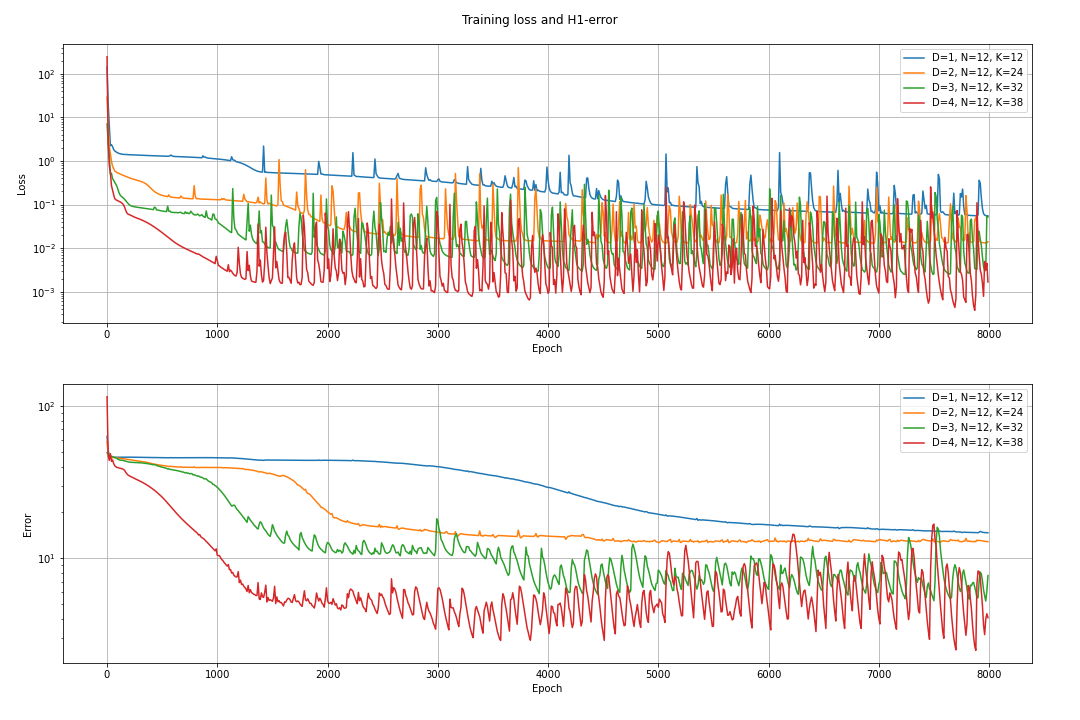
\includegraphics[width=.7\textwidth]{img/VPINN-Deep-Comparison-k8increaseD.png}
    \caption{Training loss and H1-error of a network with $N=20$ for frequency $k=8.0$, with different depths and number of test functions.}
    \label{fig:vpinnsdeepincreaseD}
\end{figure}

In \autoref{fig:vpinnsdeepincreaseD}, we keep the width of the network to $N=12$, increase the depth of the netowrk, and increase the number of test functions as $K \simeq 12\sqrt{N_p/50}$ as concluded earlier. It shows that with this approach, both the convergence speed and the final accuracy could be improved very well. Comparing this approach with the best approach in shallow neural networks (increasing the width and the number of test functions equally), we saw that on our CPUs, the deep network with $D=4$, $N=12$ and 38 test functions reaches a decent H1-error in 15 minutes, while a shallow neural network with $20$ nodes and $20$ test functions requires 65 minutes for reaching the same accuracy.
% TODO: Conclusion: It is beneficial to increase the depth (AND K) instead of the width

\subsubsection{V-elliptic Formulation}\label{seq:velliptic}


\section{Conclusion}\label{sec:conclusion}
% TODO: Suggestions for future work
% TODO: Add something innovative
